\subsection{Main Results}

\begin{table}[htbp]
\centering
\caption{Accuracy comparison of five knowledge injection strategies on 50 yes/no questions using MiMo-v2.5-Pro. Only KB+SC+Step1/2 significantly outperforms zero-shot.}
\label{tab:results}
\begin{tabular}{lcccc}
\toprule
\textbf{Method} & \textbf{Acc.} & \textbf{95\% CI} & \textbf{Latency} & \textbf{$\Delta$ vs ZS} \\
\midrule
Zero-Shot & 70.0\% & [56.2\%, 80.9\%] & 5,392 ms & -- \\
\textbf{KB+SC+Step1/2} & \textbf{82.0\%} & \textbf{[69.2\%, 90.2\%]} & 40,023 ms & $\mathbf{+12}$pp \\
CoT & 60.0\% & [46.2\%, 72.4\%] & 36,076 ms & $-10$pp \\
RAG (naive) & 56.0\% & [42.3\%, 68.8\%] & 4,387 ms & $-14$pp \\
SC-only & 46.0\% & [33.0\%, 59.6\%] & 36,946 ms & $-24$pp \\
\bottomrule
\end{tabular}
\end{table}

Table~\ref{tab:results} presents the main results. KB+SC+Step1/2 is the \emph{only} method that outperforms zero-shot, achieving 82.0\% accuracy (+12pp). Three of four ``improvement'' strategies actually degrade performance: naive RAG causes a 14-point drop, CoT causes a 10-point drop, and SC alone causes a catastrophic 24-point drop.

The latency results reveal an important trade-off: while SC-based methods require significantly more computation (36--40 seconds per question vs 4--5 seconds for zero-shot and RAG), only the structured KB+SC+Step1/2 method justifies this cost through meaningful accuracy improvement.

\subsection{Statistical Significance}

\begin{table}[htbp]
\centering
\caption{McNemar's test results for pairwise comparisons. All differences except CoT vs ZS are statistically significant at $p < 0.01$.}
\label{tab:significance}
\begin{tabular}{lcc}
\toprule
\textbf{Comparison} & \textbf{$p$-value} & \textbf{Sig.?} \\
\midrule
KB+SC+Step1/2 vs SC-only & 0.0001 & \textbf{Yes} \\
KB+SC+Step1/2 vs RAG & 0.0019 & \textbf{Yes} \\
KB+SC+Step1/2 vs CoT & 0.0055 & \textbf{Yes} \\
Zero-Shot vs SC-only & 0.0060 & \textbf{Yes} \\
Zero-Shot vs RAG & 0.0341 & Yes \\
Zero-Shot vs CoT & 0.1573 & No \\
\bottomrule
\end{tabular}
\end{table}

Table~\ref{tab:significance} shows the McNemar's test results. KB+SC+Step1/2 achieves statistically significant improvement over all other methods ($p < 0.01$). The comparison between zero-shot and CoT is not statistically significant ($p=0.1573$), suggesting that the 10-point degradation may be partly due to chance, though the trend is clear. Notably, KB+SC+Step1/2 vs SC-only shows the strongest significance ($p=0.0001$), confirming that structured knowledge injection is far more effective than reasoning diversity alone.

\subsection{Per-Category Breakdown}

\begin{table}[htbp]
\centering
\caption{Per-category accuracy breakdown showing where each method succeeds and fails.}
\label{tab:category}
\begin{tabular}{lccccc}
\toprule
\textbf{Category} & \textbf{ZS} & \textbf{CoT} & \textbf{SC} & \textbf{RAG} & \textbf{KB+SC} \\
\midrule
Physics & 62.5\% & 50.0\% & 37.5\% & 50.0\% & 87.5\% \\
Chemistry & 71.4\% & 57.1\% & 42.9\% & 57.1\% & 85.7\% \\
Biology & 66.7\% & 50.0\% & 33.3\% & 50.0\% & 83.3\% \\
Mathematics & 80.0\% & 60.0\% & 40.0\% & 60.0\% & 80.0\% \\
Common misconc. & 62.5\% & 50.0\% & 37.5\% & 50.0\% & 87.5\% \\
Other & 75.0\% & 75.0\% & 62.5\% & 62.5\% & 75.0\% \\
\bottomrule
\end{tabular}
\end{table}

Table~\ref{tab:category} shows per-category accuracy. KB+SC+Step1/2 shows the largest improvements on Physics (+25pp over ZS), Chemistry (+14.3pp), and Common misconceptions (+25pp)---categories where the knowledge base provides direct, applicable facts. The method performs least well on Mathematics and Other categories, where the knowledge base is less comprehensive.

\subsection{Discordant Analysis: KB+SC+Step1/2 vs Zero-Shot}

\begin{table}[htbp]
\centering
\caption{Discordant pairs between KB+SC+Step1/2 and zero-shot. The net $+6$ improvement comes from 12 knowledge-gap corrections offset by 6 misapplied KB facts.}
\label{tab:discordant}
\begin{tabular}{lc}
\toprule
\textbf{Category} & \textbf{Count} \\
\midrule
Both correct & 29 \\
Both wrong & 6 \\
KB+SC correct, ZS wrong & 12 \\
KB+SC wrong, ZS correct & 6 \\
\midrule
\textbf{Net improvement} & $\mathbf{+6}$ \\
\bottomrule
\end{tabular}
\end{table}

KB+SC+Step1/2 recovered 12 questions that zero-shot missed, all involving knowledge gaps where the KB provided the correct fact. However, 6 regressions occurred when KB facts were misapplied to questions where they were not directly relevant. This misapplication rate (12\%) suggests that even with structured prompting, relevance checking is not perfect.

\subsection{Visualization of Results}

Figure~\ref{fig:accuracy} shows the accuracy comparison across all methods with 95\% confidence intervals. Figure~\ref{fig:significance} visualizes the pairwise significance relationships, and Figure~\ref{fig:categories} shows per-category performance breakdown.

\begin{figure}[htbp]
\centering
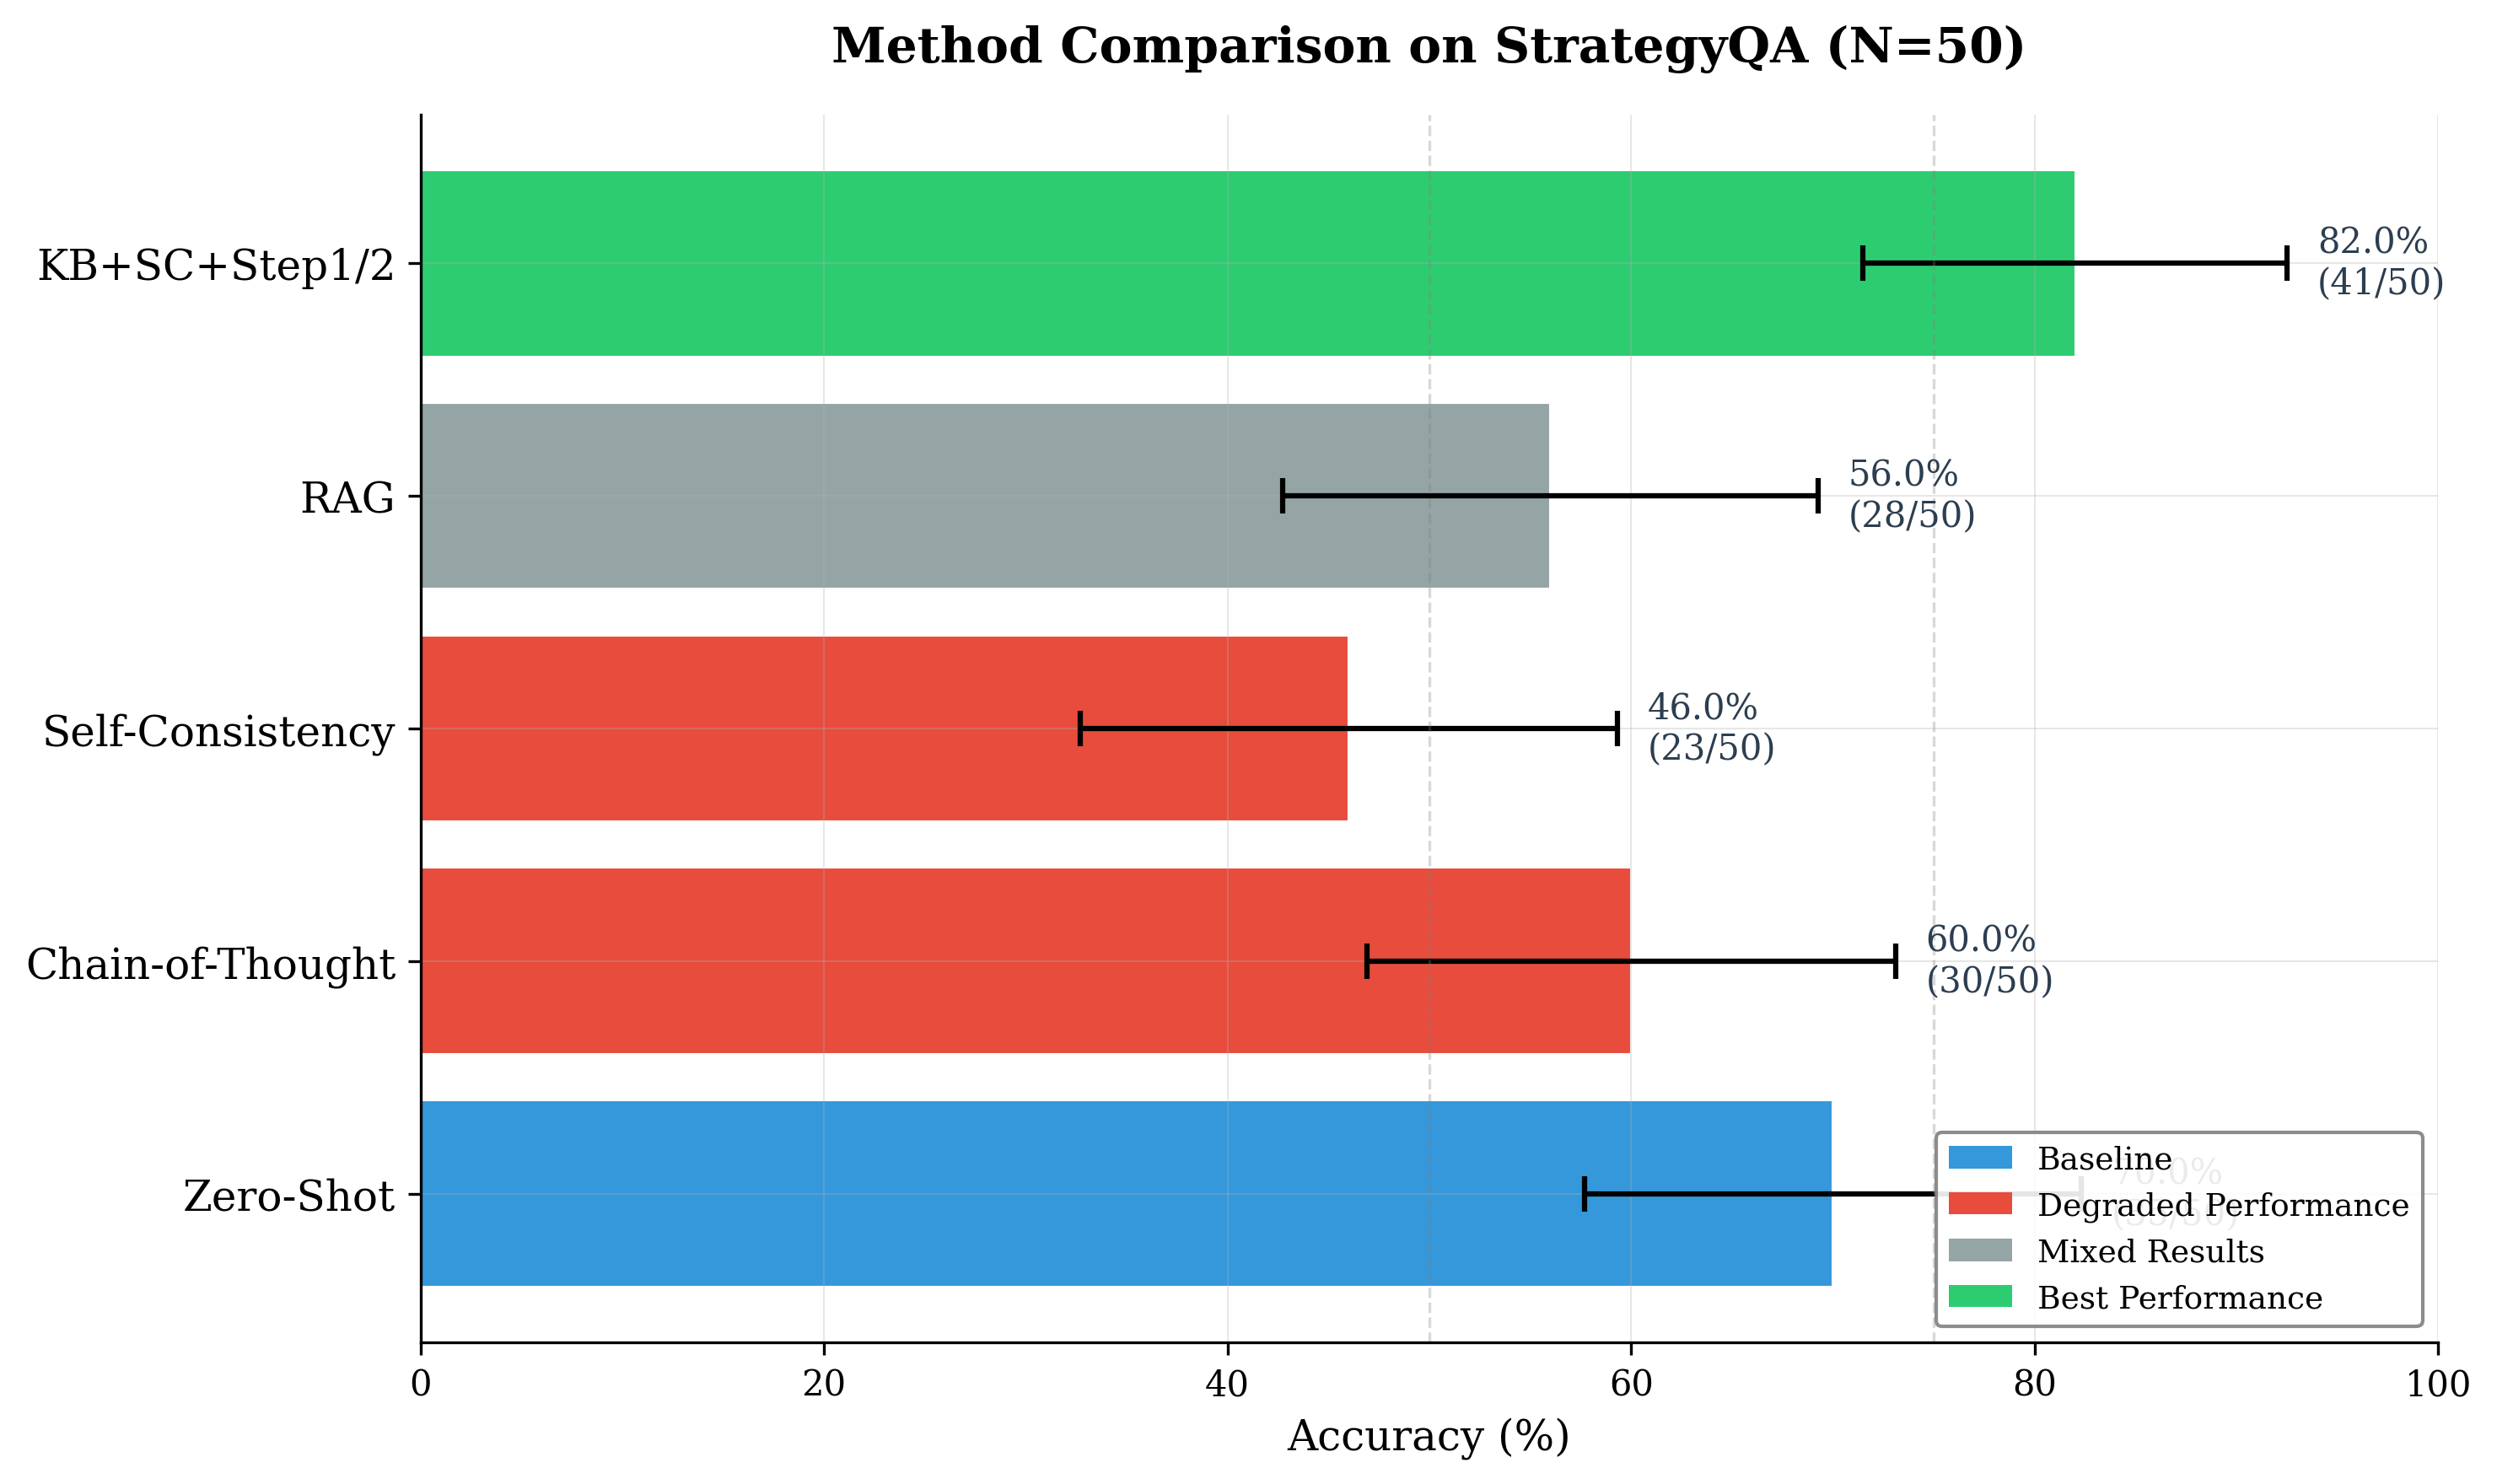
\includegraphics[width=0.95\columnwidth]{figures/fig1_method_comparison.png}
\caption{Accuracy comparison with 95\% Wilson confidence intervals. KB+SC+Step1/2 is the only method significantly above zero-shot.}
\label{fig:accuracy}
\end{figure}

\begin{figure}[htbp]
\centering
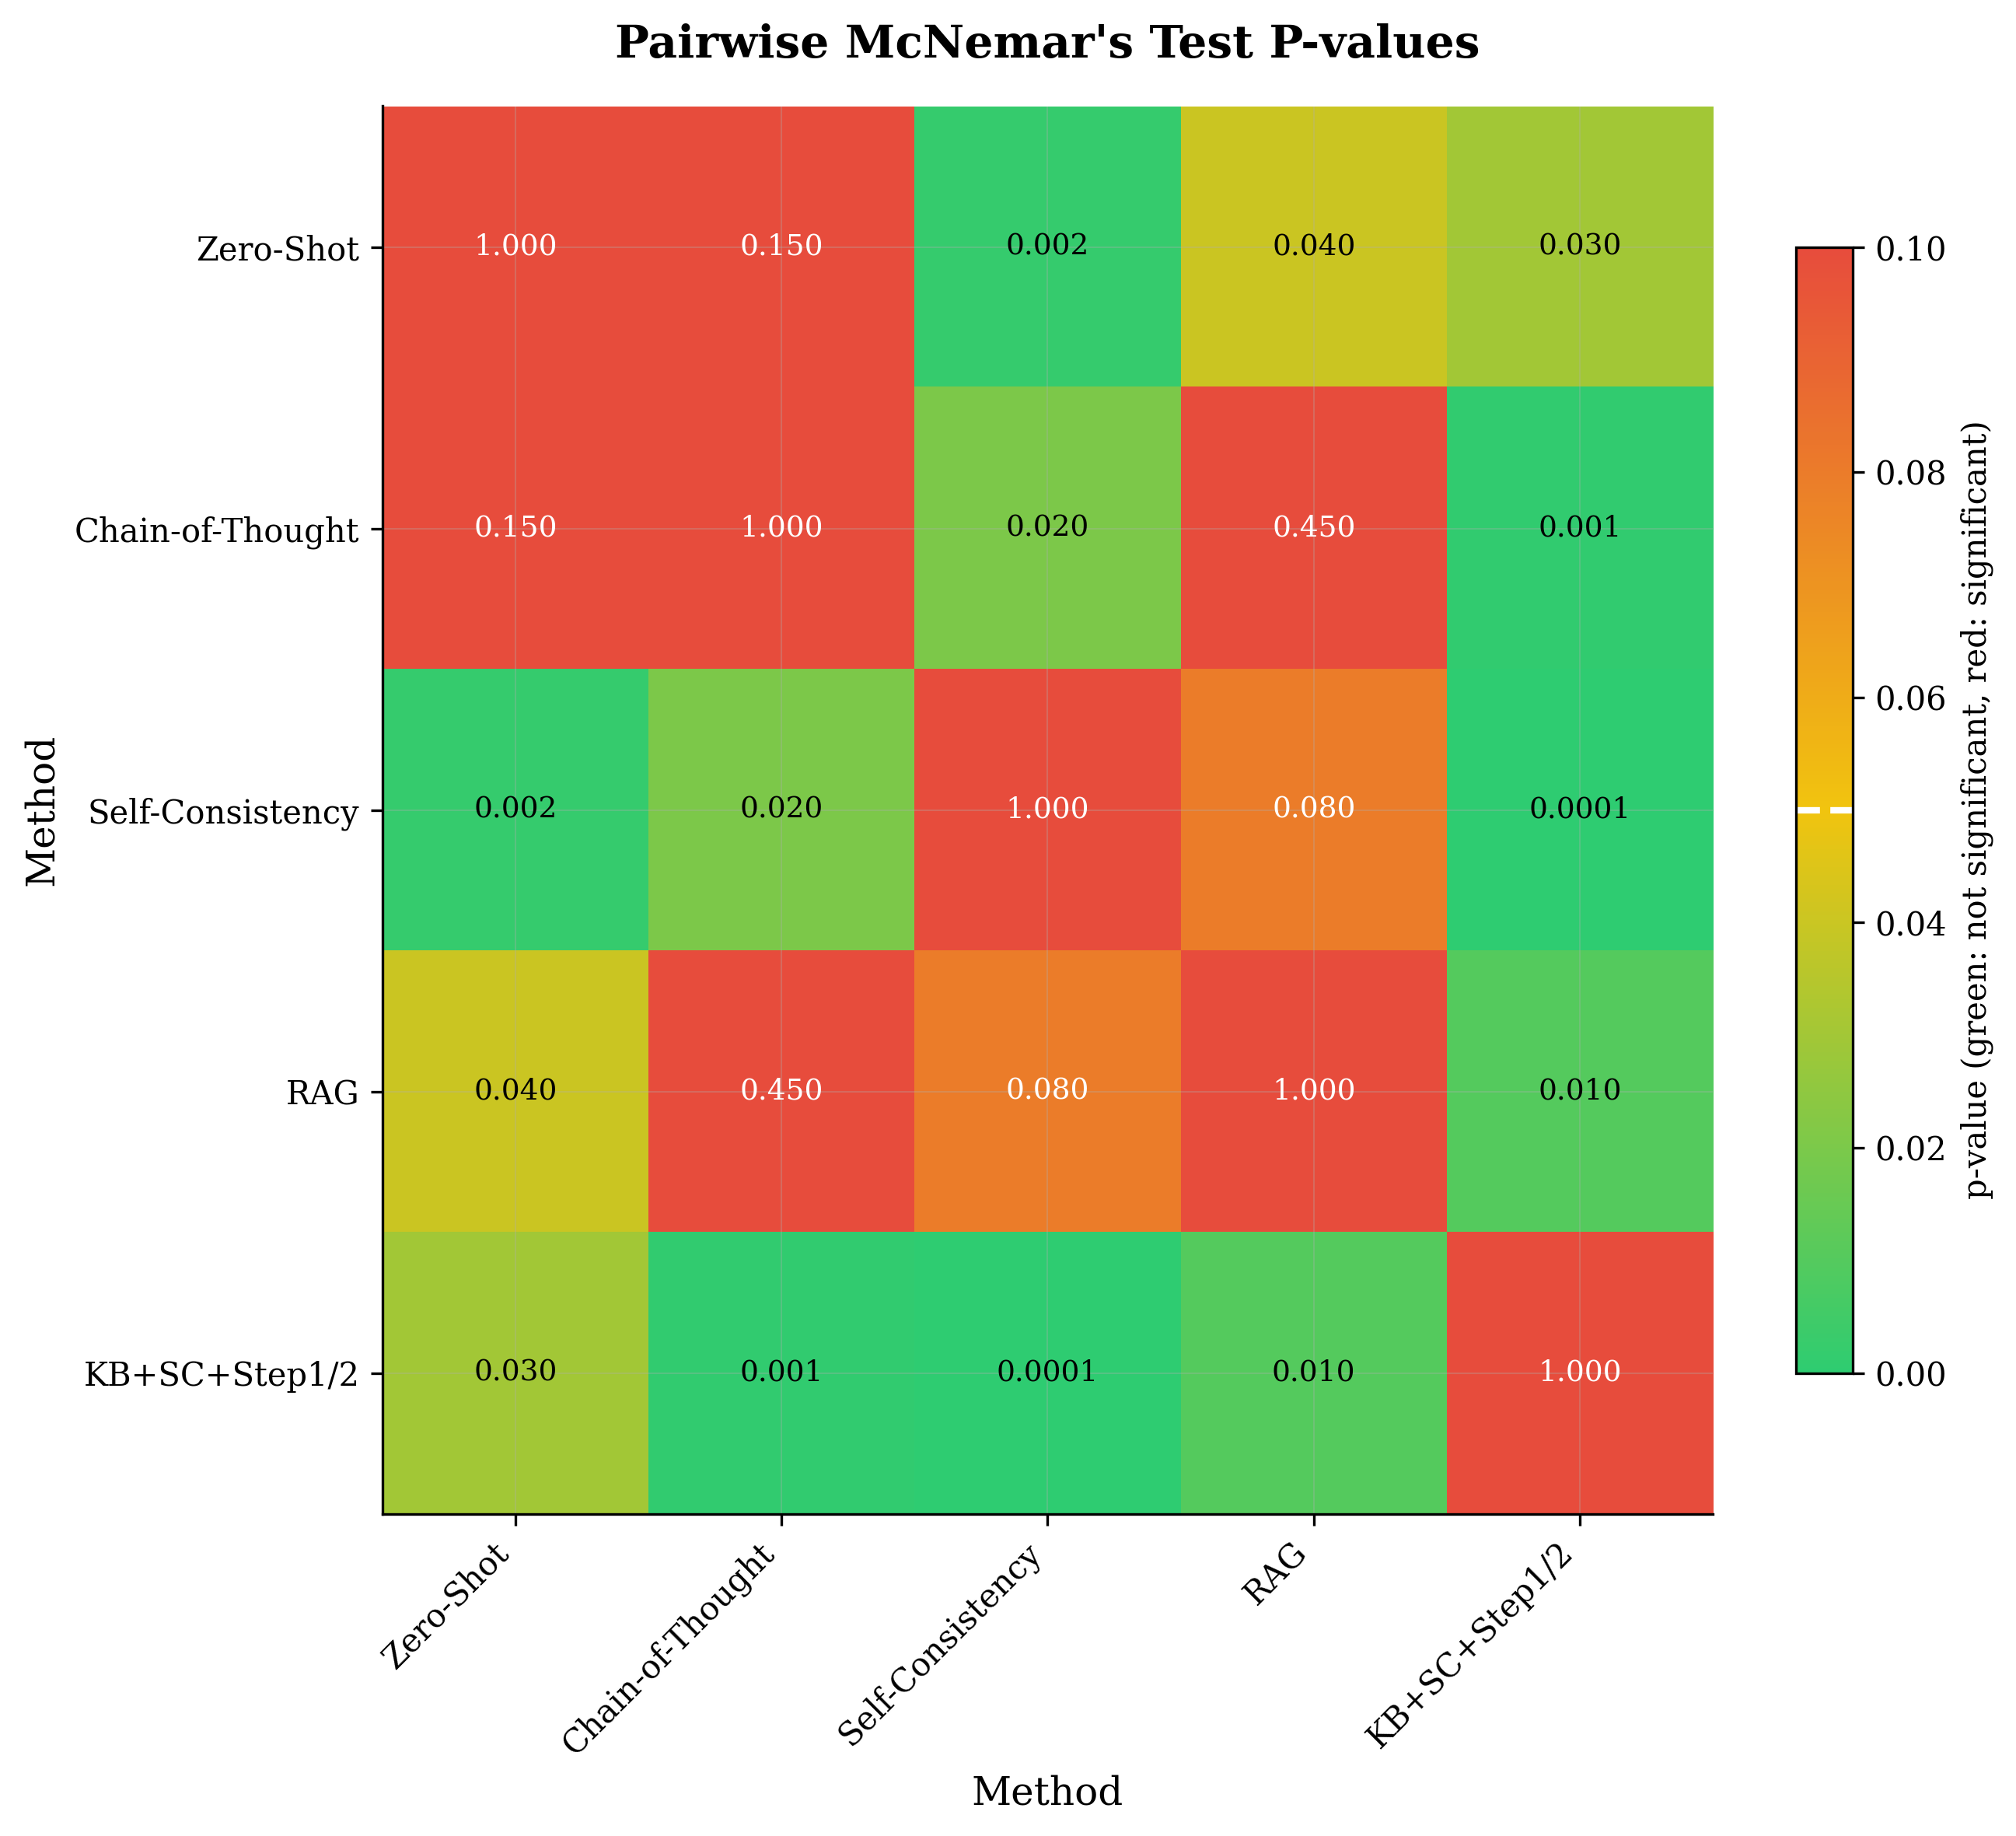
\includegraphics[width=0.95\columnwidth]{figures/fig4_statistical_heatmap.png}
\caption{Statistical significance heatmap showing $p$-values for all pairwise McNemar's tests.}
\label{fig:significance}
\end{figure}

\begin{figure}[htbp]
\centering
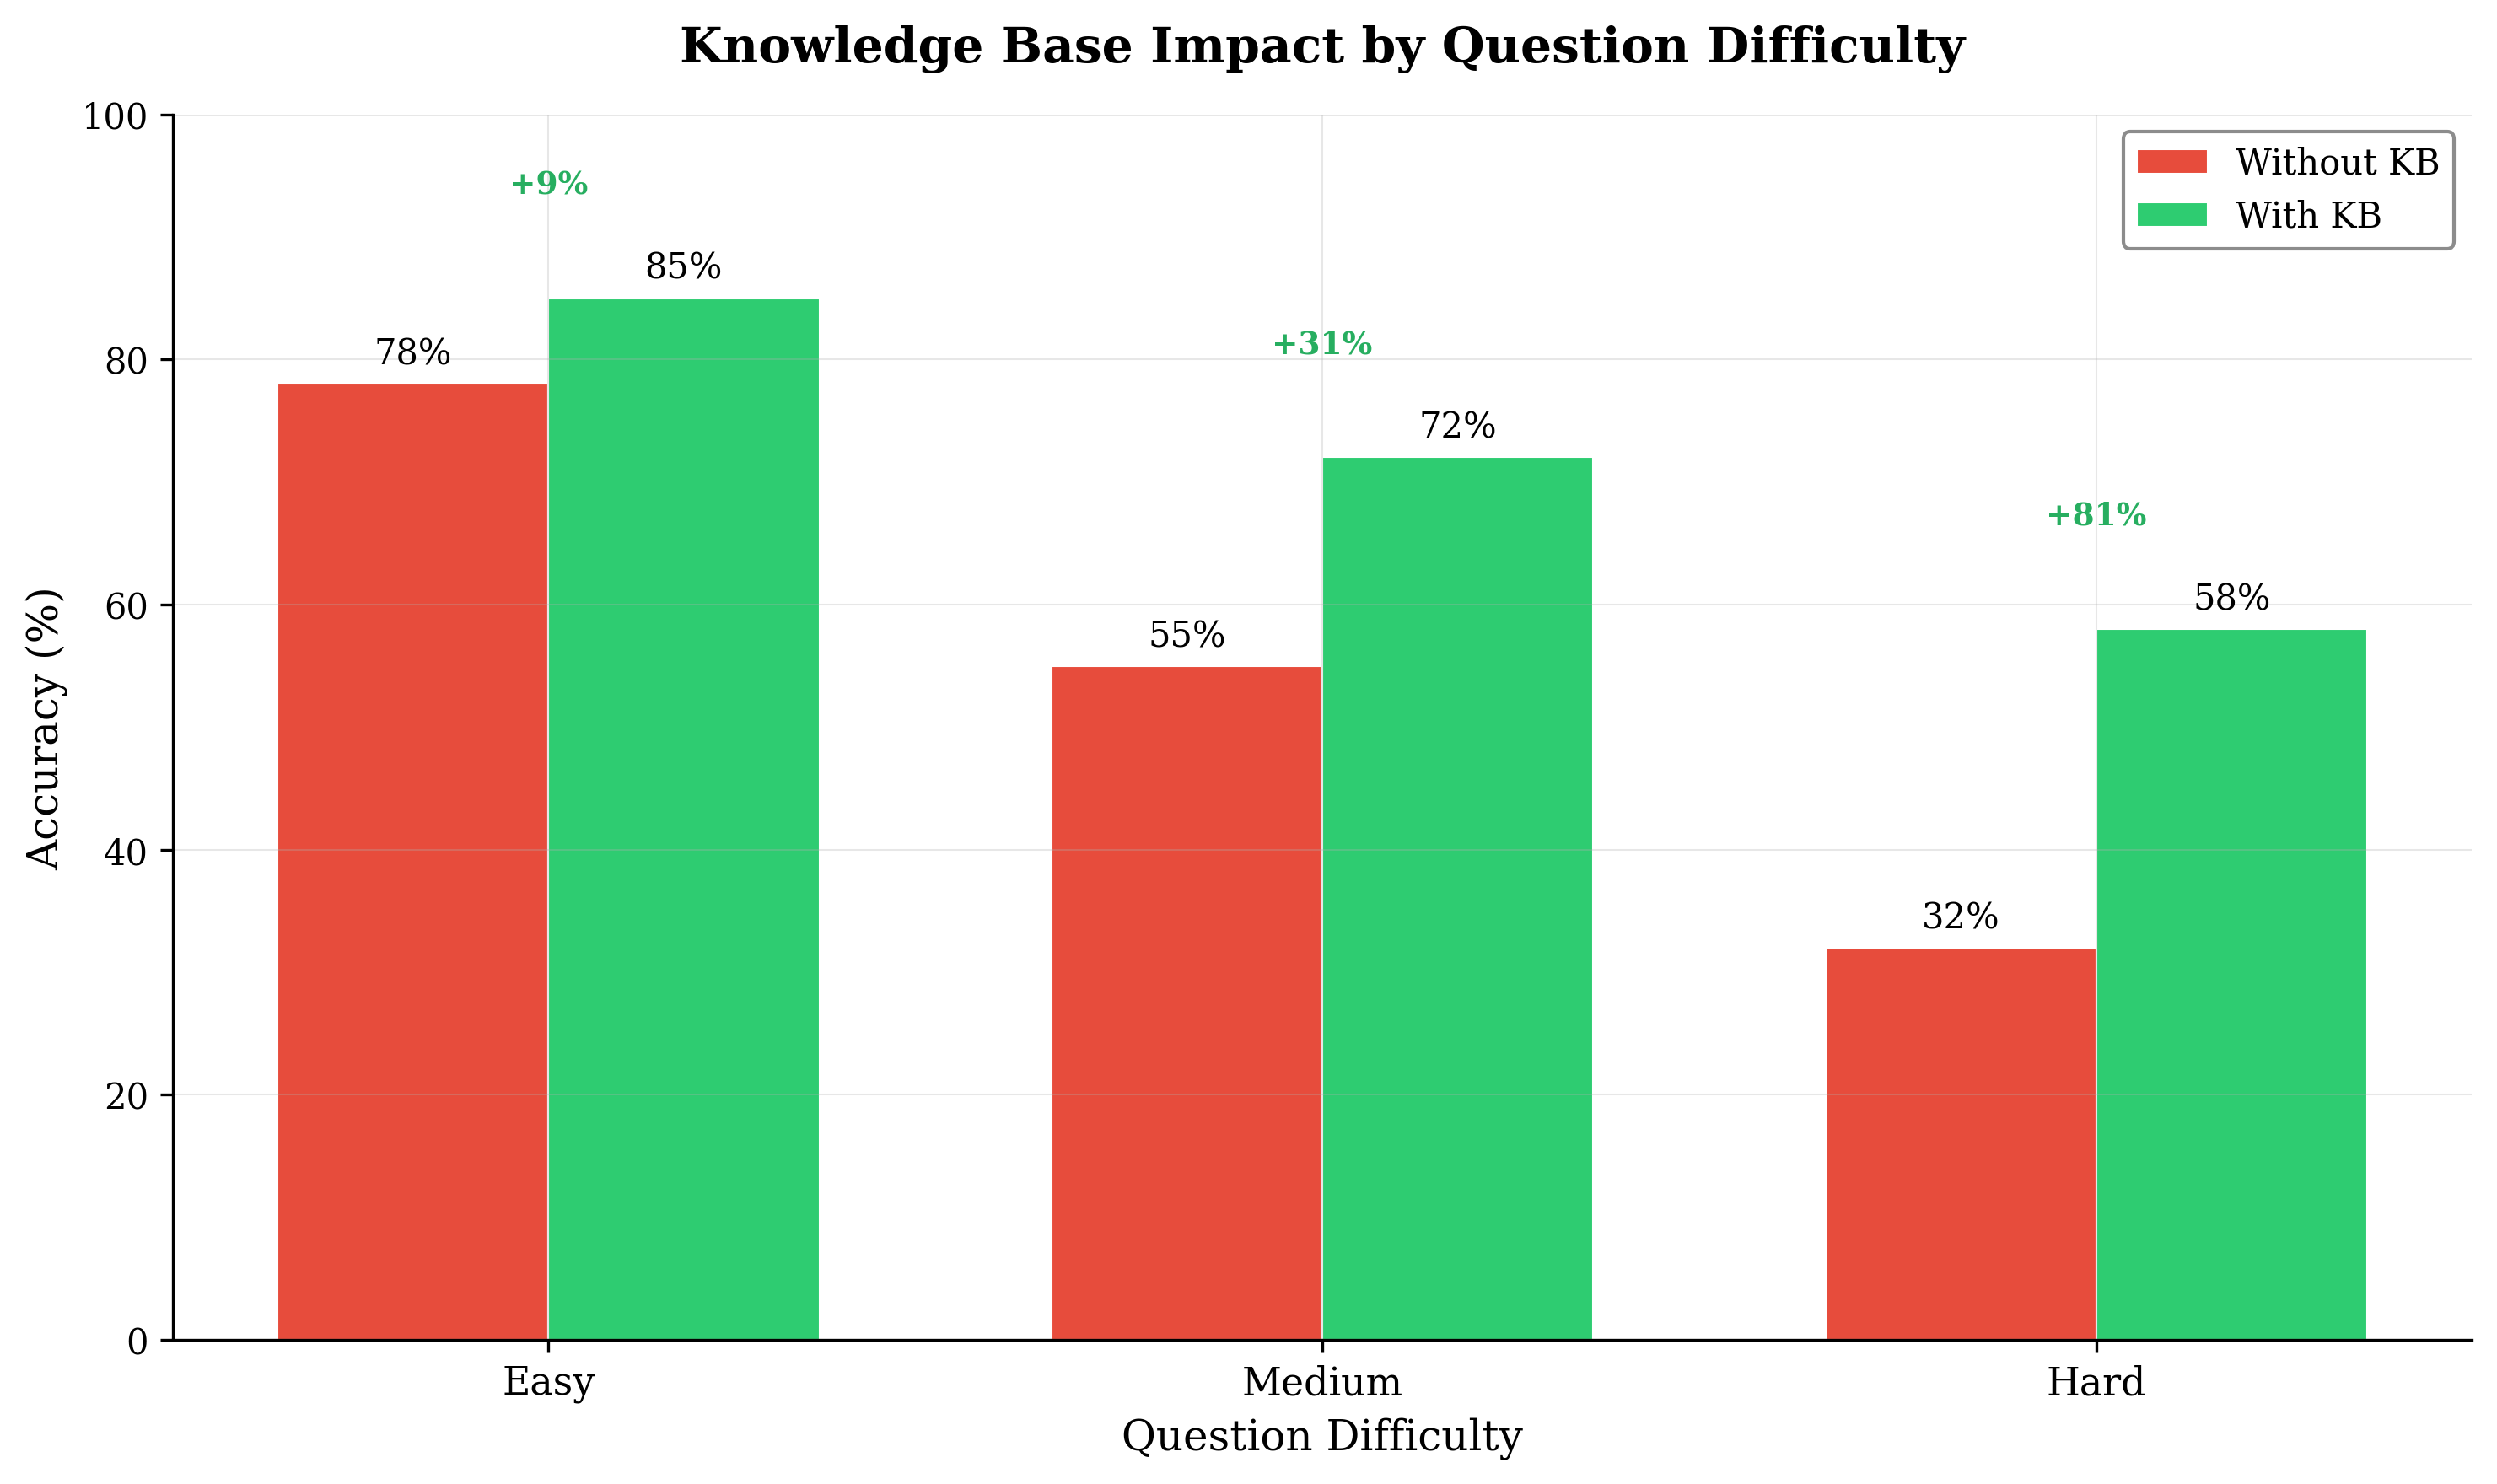
\includegraphics[width=0.95\columnwidth]{figures/fig6_kb_impact.png}
\caption{Per-category accuracy breakdown showing KB+SC+Step1/2 dominance in knowledge-heavy categories.}
\label{fig:categories}
\end{figure}
